\documentclass{book}
\usepackage{graphicx}
\usepackage{hyperref}
\usepackage{bookmark}
\usepackage[T1]{fontenc}
\usepackage[framed, numbered]{matlab-prettifier}
\lstset{basicstyle=\mlttfamily, style=Matlab-editor, escapechar=`}
\newcommand{\ml}[1]{\lstinline{#1}}
\author{Bart Vermeulen}
\title{ADCPtools}

\begin{document}
\maketitle
\chapter{Getting started}
\section{Getting help}
To get an overview of all the functions in adcptools run
\begin{lstlisting}
help `\mlplaceholder{Path to adcptools}`
\end{lstlisting}
This will display all the avilable functions and clicking on the function name will display the help of the function.

\section{Vessel mounted ADCP data processing}
The procedure described in this section can also be found in the ``demo'' folder under the ``doc'' foloder, including some raw data.

To process vessel mounted ADCP data, it is convenient to store all the collected data files from one deployment into a folder.
The data can be read with the following line:
\begin{lstlisting}
data=readDeployment(depName, path)
\end{lstlisting}
in which \ml{depName} is the deployment name (i.e. the common part of the files to be read) and \ml{path} the folder where the files are located.
The output is a structure that can contains all the data.

To check the path sailed by the vessel \autoref{fig:track}:
\begin{lstlisting}
[x,y]=utmADCP(data);
plot(x,y)
axis equal
\end{lstlisting}

\begin{figure}[h]
  \centering
  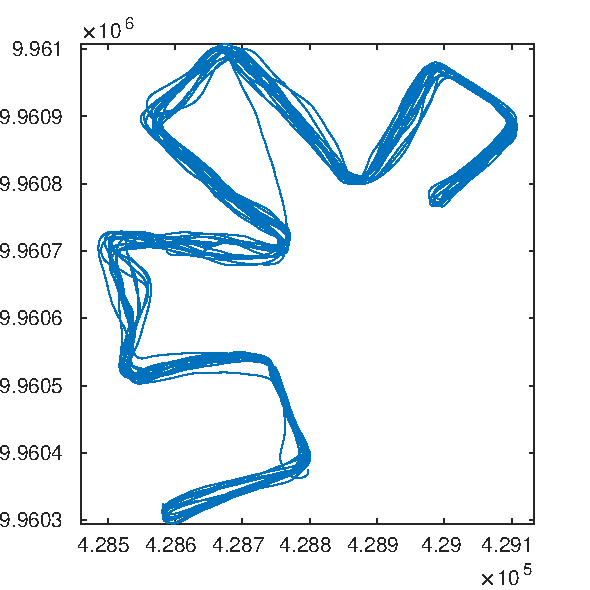
\includegraphics{figures/track.pdf}
  \caption{Plotting the track sailed by the ADCP}
  \label{fig:track}
\end{figure}

To process repeat transect data, it is necessary to first define which ensembles belong to a specific cross section and and to a certain crossing. 
This is done using the \ml{tid} matrix \autoref{fig:tid}. Each column in the matrix represent an ensemble and each row a cross-section. The number in the matrix indicates to which repeat the ensemble belongs to. A zero indicates the ensemble does not belong to the cross-section. In other words if \ml{tid(3,15)=1}, it indicates that the 15th ensemble is part of the first repeat-transect on cross-section 3. Note that an ensemble can be part of different cross-sections, which might be the case when the cross-sections intersect.
\begin{figure}[h]
	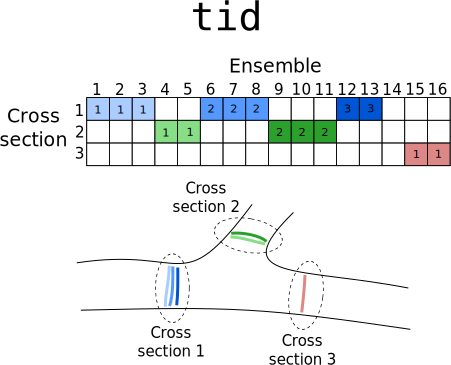
\includegraphics[width=\linewidth]{figures/tid.pdf}
	\caption{Example of a \ml{tid} matrix. Three cross-section are defined and for each transect different repeat-transect are distinguished. White elements in the matrix indicate zero value.}
	\label{fig:tid}
\end{figure}

Once the \ml{tid} matrix has been defined, the velocity data can be processed using the \ml{procTrans} function.
\begin{lstlisting}
msh=procTrans(data,tid)
\end{lstlisting}
This calls the \ml{procTrans} function that will process the ADCP data in the structure \ml{data} and with the cross-sections and the repeat transects defined in the matrix \ml{tid}. 

The output structure \ml{msh} contains for each cross-section the mesh on which the velocity data were averaged, and the output velocity. The coordinates of the cell centers are found in the \ml{msh.X},\ml{msh.Y}, \ml{msh.Z}, \ml{msh.N}. The velocity can be found in the array \ml{msh.pars}. The name stems from the used velocity model. In this case it is assumed that the velocity is a constant value in each cell. This can be replaced with e.g. a Taylor expansion, or a simple tidal model. For further details on input parameters and output format see the help of the \ml{procTrans} function.
\begin{lstlisting}
%% Make simple velocity plot
figure
cs=3;  % select cross section
rot='cs'; % select velocity rotation
imagesc(msh(cs).(rot).pars(:,:,end,1)) % quickly show longitudinal velocity
\end{lstlisting}
Plotting the results can be done easily using e.g. \ml{imagesc} (\autoref{fig:quick_view}).
\begin{figure}[p]
  \centering
  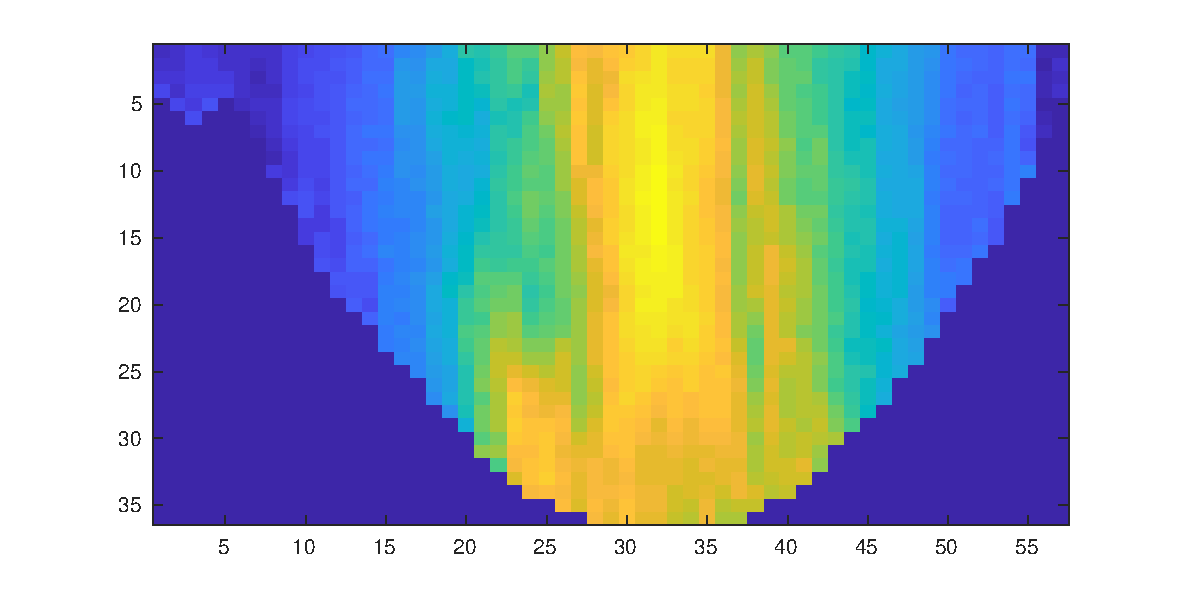
\includegraphics[width=\linewidth]{figures/simple_plot.pdf}
  \caption{Quick view of longitudinal velocity}
  \label{fig:quick_view}
\end{figure}
A prettier figure can be made using the \ml{msh.p} structure, which contain the outlines of the mesh cells and variables (starting with \ml{progfgood}) to select the velocity values corresponding to the mesh cells \autoref{fig:fancy_plot}:
\begin{lstlisting}[basicstyle=\mlttfamily\small]
%% Make fancy velocity plot (using p structure in output mesh)
figure
cs=3;% select cross section
rot='cs';% select velocity rotation
qscale=20;% set secondary flow quiver scaling

patch(msh(cs).p.N,...% n-coordinate of cell edges
      msh(cs).p.Z(:,:,end),...% z-coordinate of cell edges (end: selects average over all repeats)
      msh(cs).(rot).pars(msh(cs).p.progfgood_vec(:,end,1)))% longitudinal flow (used progfgood to select only values inside mesh
shading flat% remove edges of cells
set(gca,'clim',[-0.3 0.6]) % set color limits of figure
colormap(flipud([103,0,31; % set a colormap (based on colorbrewer)
178,24,43;  
214,96,77;
244,165,130;
253,219,199;
247,247,247;
247,247,247;
209,229,240;
146,197,222])/255)
cb=colorbar; % add a colorbar
hold on  % add next plots
plot(msh(cs).p.nbed,msh(cs).p.zbed,'k','linewidth',2) % draw bed
plot(msh(cs).p.nbed([1 end]),[0 0],'b','linewidth',2) % draw water surface
quiver(...% draw secondary flow vectors
       msh(cs).N,... % n coordinate of cell centers
       msh(cs).Z(:,:,end),...% z coordinate of cell centers
       squeeze(msh(cs).(rot).pars(:,:,end,2)*qscale),...% n-velocity
       squeeze(msh(cs).(rot).pars(:,:,end,3)*qscale),...% z-velocity
       'color','k','autoscale','off') % black quivers, manually scaled

% add labels and quiver scale to plot
xlabel('n coordinate (m)')
ylabel('z coordinate (m)')
ylabel(cb,'Longitudinal velocity (m/s)')
quiver(50, -35,1*qscale,0,'k','autoscale', 'off');
quiver(50, -35, 0,0.2*qscale,'k','autoscale', 'off');
text(45,-33,'0.2 m/s','HorizontalAlignment','right')
text(60,-36,'1 m/s','HorizontalAlignment','center',...
                    'VerticalAlignment','top')
\end{lstlisting}

\begin{figure}[p]
  \centering
  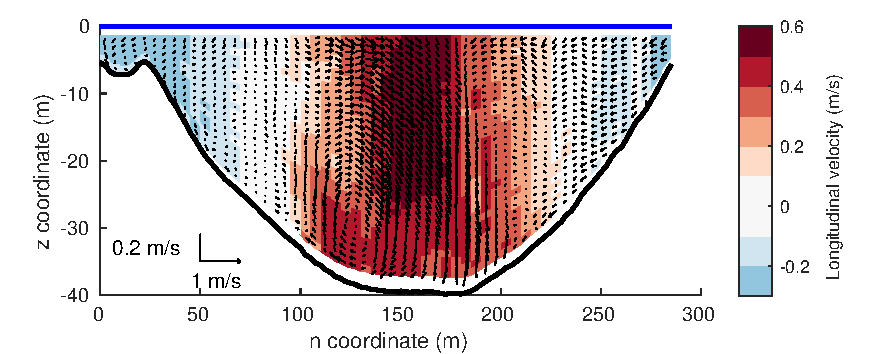
\includegraphics[width=\linewidth]{figures/proc_trans_results.pdf}
  \caption{More elaborate figure using the mesh cell boundaries defined in the \ml{msh.p} structure.}
  \label{fig:fancy_plot}
\end{figure}


\end{document}
